Sei $ABCD$ ein gleichschenkliges Trapez mit $AD>BC$. Sei $X$ der Schnittpunkt der Winkelhalbierenden von $\angle BAC$ und $BC$. Sei $E$ der Schnittpunkt von $DB$ mit der Parallelen zu der Winkelhalbiernden von $\angle CBD$ durch $X$ und sei $F$ der Schnittpunkt von $DC$ mit der Parallelen zu der Winkelhalbiernden von $\angle DCB$ durch $X$. Zeige, dass $AEFD$ ein Sehenviereck ist.

\textbf{Lösung (Patrick)}

 Da $ABCD$ ein Sehnenviereck ist, hat man $\angle ABE = \angle ACF$.
 
 Wenn man beweist, dass die Dreiecke $\triangle ABE$ und $\triangle ACF$ ähnlich sind, dann hat man, dass $\angle AED = \angle AEB = \angle AFC = \angle AFD$ also ist $AEFD$ ein Sehnenviereck.
 Man muss also nur noch zeigen, dass $\frac{AB}{BE} = \frac{AC}{CF}$.
 
Weil die Gerade EX parallel zur Winkelhalbieren ist, findet man $\angle XEB = \angle EXB$ und somit $BE = BX$ und auf genau gleiche Weise $CF = CX$.

Die Dreiecke $AFC$ und $AEB$ sind also genau dann ähnlich zueinander, wenn $\frac{AB}{BX} = \frac{AC}{CX}$. 
Diese Gleichung findet man aber mit dem magischen Lemma oder mit ähnlichen Dreiecken, da $X$ der Schnittpunkt der Winkelhalbierenden von $\angle BAC$ mit $BC$ ist.

\begin{center}
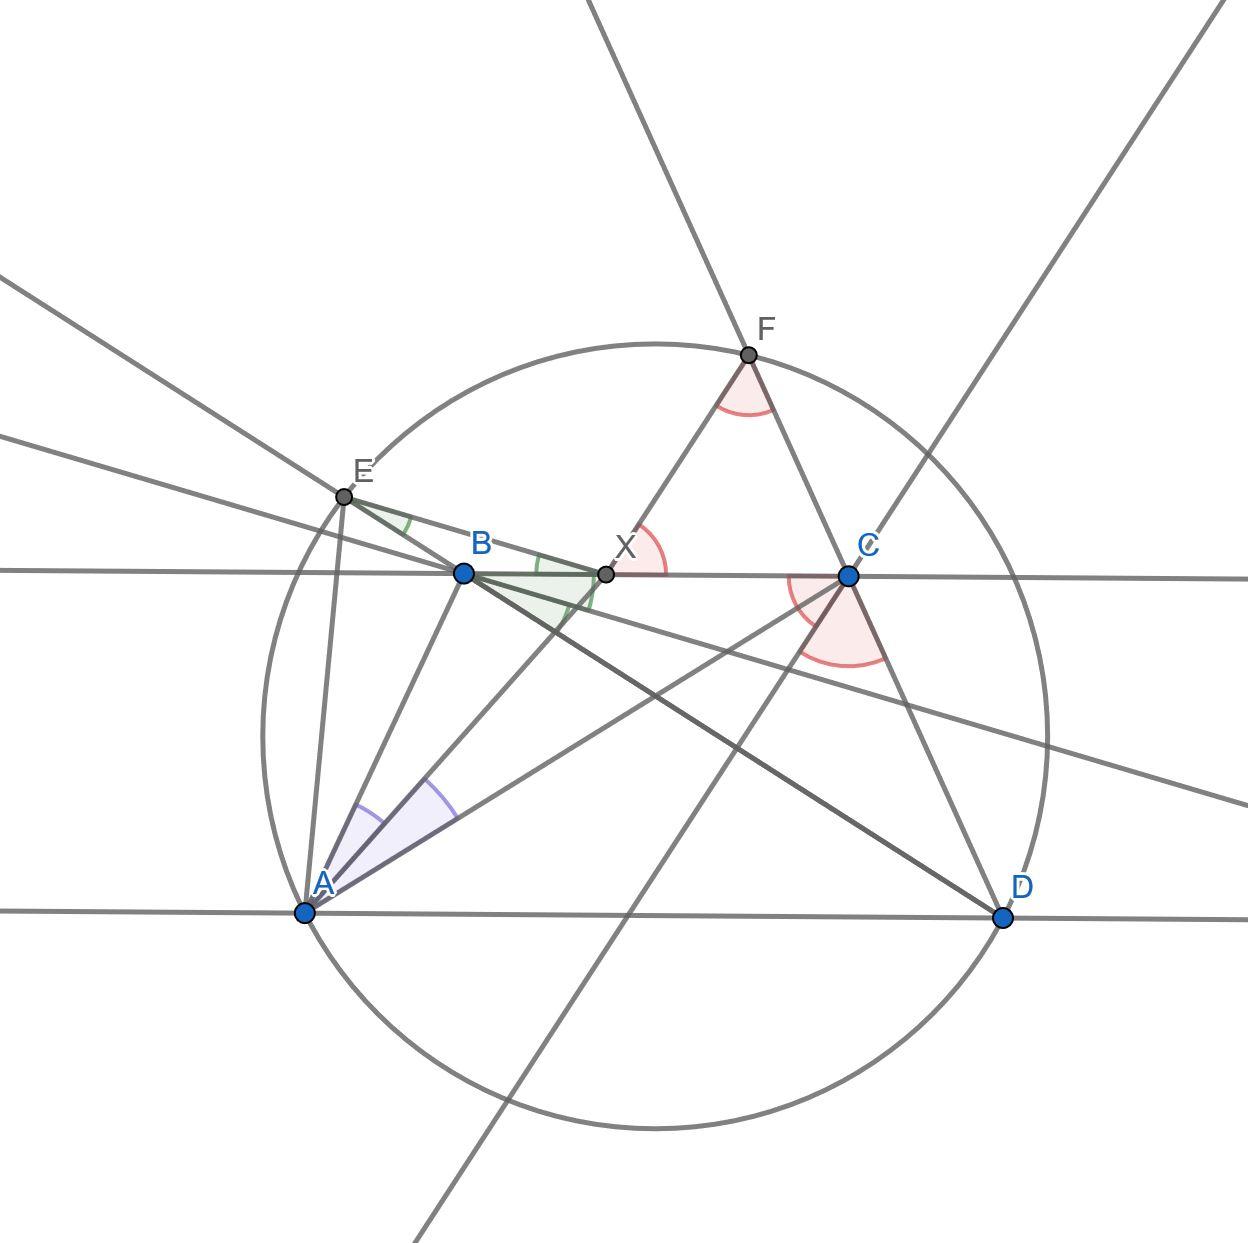
\includegraphics[trim={3cm 1cm 1cm 3.5cm}, clip, width =0.65\textwidth]{f7_picture.JPG}
\end{center}

\textbf{Marking scheme} 
\begin{enumerate}

\item 1P: Aufschreiben, dass $\angle BXE = \angle BEX$, $\angle CXF = \angle CFX$ oder $\angle ABE = ACF$.
\item 1P: Zeige, dass $CF=CX$, $BE= BX$ und $\angle ABE = ACF$.
\item 1P: Aufschreiben, dass $\frac{AB}{BX} = \frac{AC}{CX}$.
\item 1P: Aufschreiben, dass $\frac{AB}{BE} = \frac{AC}{FC}$.
\item 1P: Beweise, dass $AFC$ ähnlich zu $AEB$. 
\item 2P: Feststellen, dass es ausreicht zu zeigen, dass $AFC$ und $AEB$ ähnlich zueinander sind. 

   
\end{enumerate}{}